El presente capítulo presenta los resultados experimentales obtenidos al evaluar el rendimiento y desempeño del aprendizaje de tres paradigmas de inteligencia artificial: PPO \cite{schulman2017ppo}, NEAT \cite{stanley2002neat} y Decision Trees destilados \cite{breiman1984classification}. Se analizan, en primer lugar, los costos del proceso de aprendizaje (datos requeridos, tiempo de entrenamiento, recursos computacionales) para evaluar la viabilidad de cada paradigma bajo distintas condiciones de ejecución. En segundo lugar, se presentan las métricas de desempeño de los sistemas adaptativos resultantes. La combinación de ambos análisis permite determinar la factibilidad del aprendizaje en hardware local y la pertinencia de la adaptación por selección de especialistas como alternativa al entrenamiento en tiempo real.

\section{Diseño Experimental}

Los experimentos fueron diseñados con el objetivo de comparar agentes bajo condiciones idénticas, garantizando reproducibilidad y control de variables. El hardware utilizado fue un equipo de escritorio con procesador Intel de 12 núcleos lógicos, GPU NVIDIA GTX 1660 (6 GB VRAM), 16 GB de RAM y sistema operativo Windows 11.

Cada configuración experimental se ejecutó con los siguientes parámetros:

\begin{itemize}
    \item Semilla fija (\texttt{seed=123}) para reproducibilidad.
    \item Número fijo de partidas por evaluación (2,000 a 5,000 según el experimento).
    \item Mismo entorno \texttt{KnucklebonesEnv} como fuente única de verdad.
    \item Registro estructurado por turno y por partida.
\end{itemize}

Los oponentes heurísticos utilizados como benchmark fueron:

\begin{itemize}
    \item \textbf{Greedy}: maximiza el puntaje inmediato.
    \item \textbf{Denial}: prioriza destruir fichas del oponente.
    \item \textbf{Spread}: distribuye fichas entre columnas de forma equilibrada.
\end{itemize}

\section{Entrenamiento de Modelos}

Se entrenaron 10 modelos: 3 PPO, 3 NEAT y 3 DT destilados (uno por cada oponente heurístico), más un perfilador KMeans compartido. La Tabla \ref{tab:training_times} presenta los tiempos de entrenamiento y tamaños resultantes.

\begin{table}[H]
\centering
\caption{Tiempos de entrenamiento y tamaño de modelos}
\begin{tabular}{llrrl}
\hline
\textbf{Familia} & \textbf{Oponente} & \textbf{Tiempo (s)} & \textbf{Tamaño (KB)} & \textbf{Método} \\
\hline
PPO  & denial  & 1,369  & 162 & 4 envs paralelos \\
PPO  & spread  & 390    & 162 & 4 envs paralelos \\
PPO  & greedy  & 400    & 162 & 4 envs paralelos \\
NEAT & denial  & 1,995  & 2.4 & Multi-seed real (3 seeds) \\
NEAT & spread  & 1,868  & 4.2 & Multi-seed real (3 seeds) \\
NEAT & greedy  & 1,818  & 3.6 & Multi-seed real (3 seeds) \\
DT   & denial  & 2.2    & 134 & Behavior Cloning \\
DT   & spread  & 2.0    & 153 & Behavior Cloning \\
DT   & greedy  & 2.0    & 147 & Behavior Cloning \\
KMeans & 4 estilos & 50  & ---  & k=4, ventana=6 \\
\hline
\end{tabular}
\label{tab:training_times}
\end{table}

\textbf{Observaciones clave}:

\begin{itemize}
    \item PPO requirió entre 6 y 23 minutos por especialista (400,000 timesteps) utilizando Stable-Baselines3 \cite{raffin2021sb3} con 4 entornos paralelos (\texttt{SubprocVecEnv}).
    \item NEAT requirió $\sim$30 minutos por especialista (300 generaciones $\times$ 150 genomas $\times$ 102 episodios por genoma con 3 seeds simultáneas, 10 workers paralelos) utilizando neat-python \cite{neatpython2023}. Se adoptó el enfoque multi-seed real para prevenir sobreajuste a secuencias deterministas.
    \item La destilación PPO$\to$DT fue prácticamente instantánea ($<$3 segundos) y redujo el tamaño del modelo $\sim$100$\times$ respecto al PPO original.
    \item KMeans se entrenó en menos de 1 minuto.
    \item Todos los entrenamientos se ejecutaron exclusivamente en CPU, sin requerir GPU.
\end{itemize}

Las Figuras~\ref{fig:training_times} y~\ref{fig:model_sizes} presentan de forma visual la comparativa de tiempos de entrenamiento y tamaños de modelo entre paradigmas.

\begin{figure}[H]
\centering
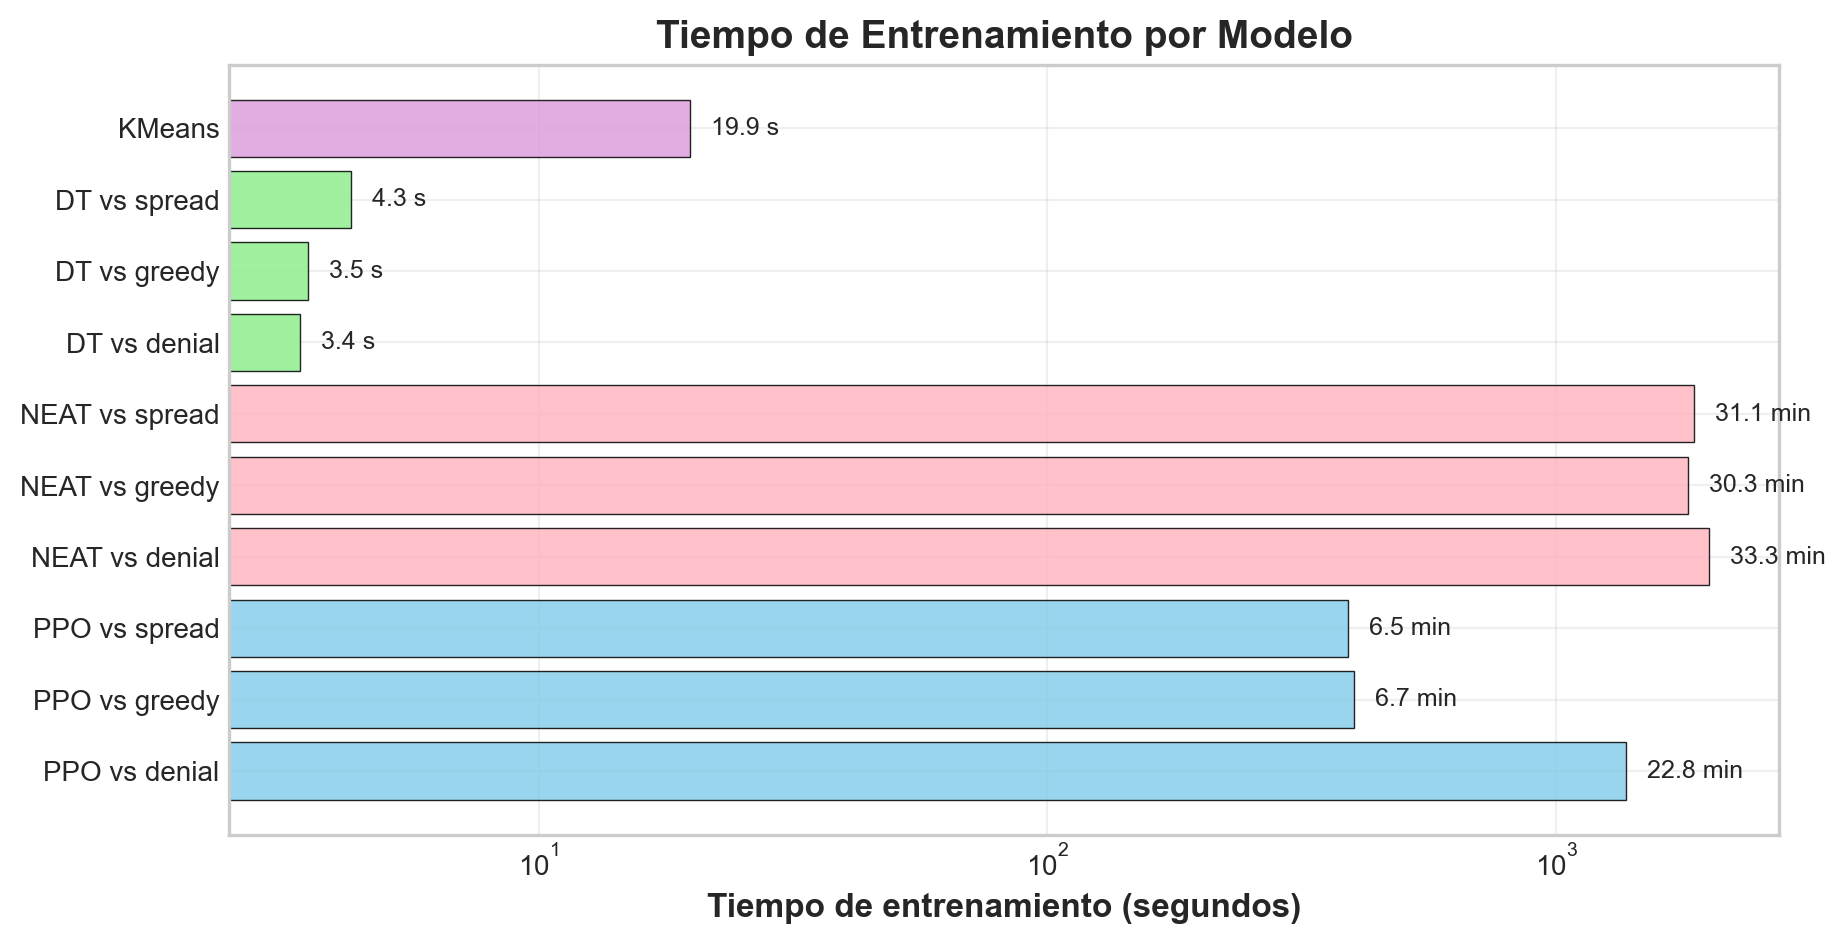
\includegraphics[width=0.75\textwidth]{figures/training_time_comparison.png}
\caption[Tiempos de entrenamiento por paradigma]{Comparativa de tiempos de entrenamiento por paradigma y oponente (escala logarítmica). NEAT requiere $\sim$30 min por especialista; PPO entre 6--23 min; DT $<$3 s por destilación.}
\label{fig:training_times}
\end{figure}

\begin{figure}[H]
\centering
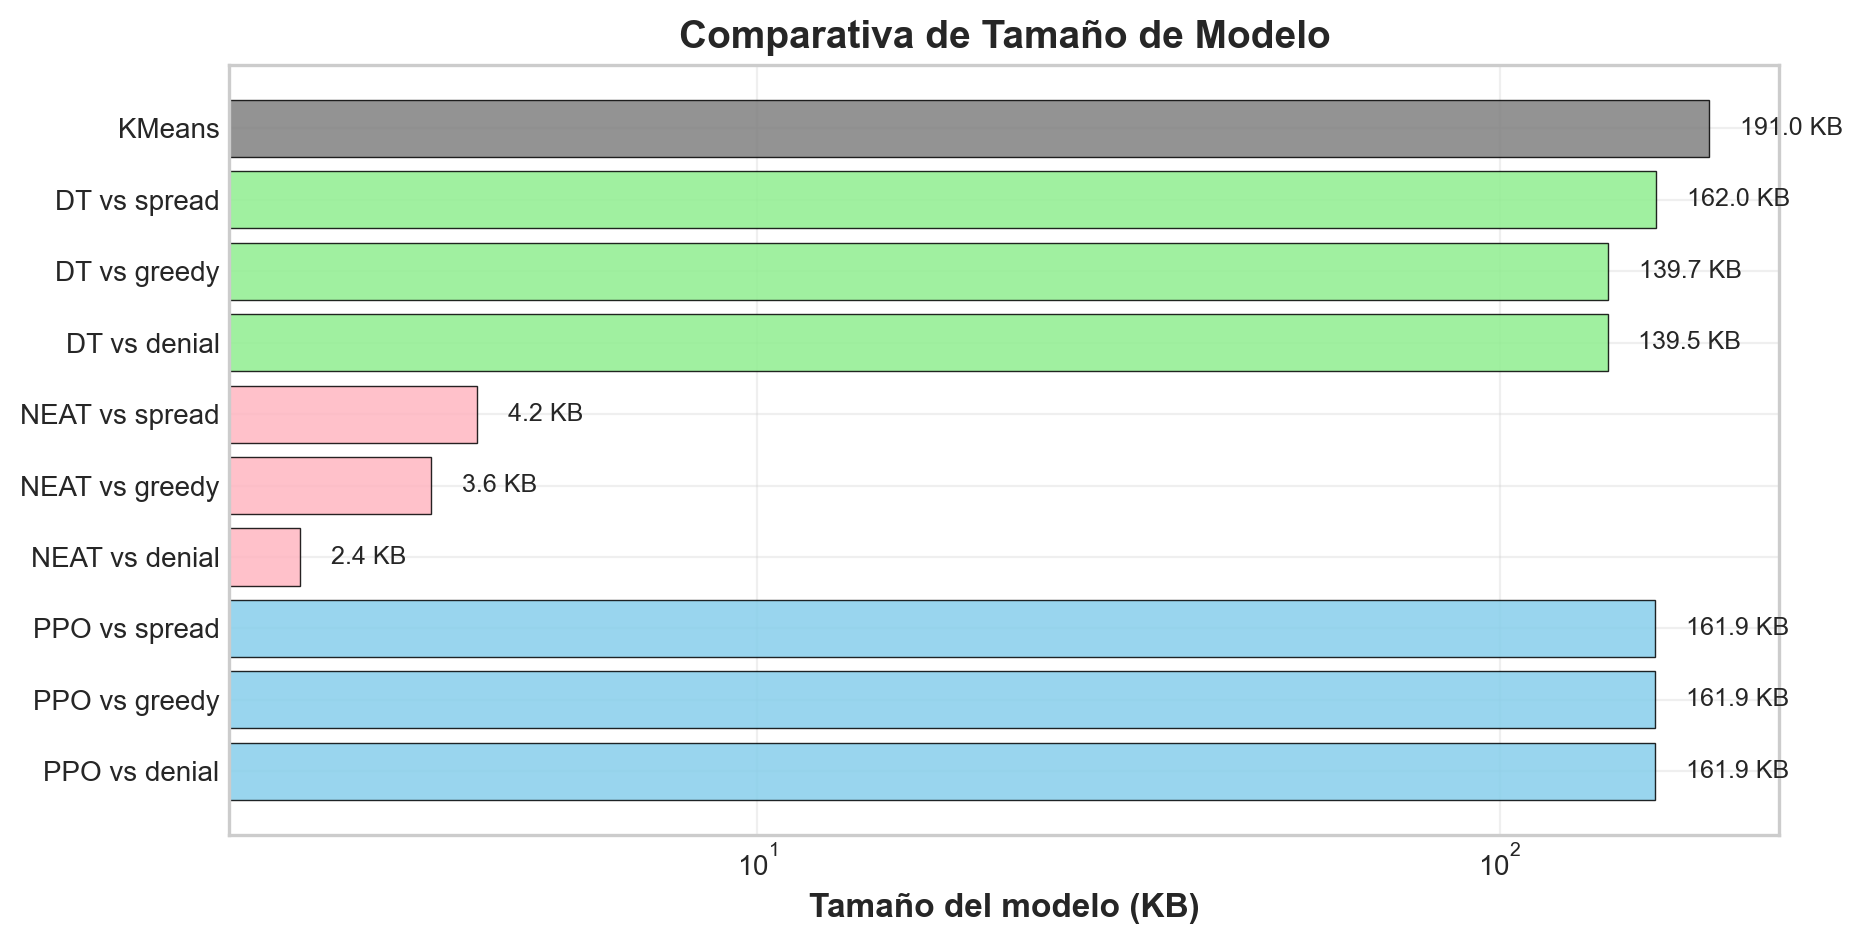
\includegraphics[width=0.75\textwidth]{figures/model_size_comparison.png}
\caption[Tamaño de modelo por paradigma]{Comparativa de tamaño de modelo resultante por paradigma (escala logarítmica). NEAT produce modelos ultraligeros ($\sim$2--4 KB); PPO $\sim$162 KB; DT $\sim$134--153 KB.}
\label{fig:model_sizes}
\end{figure}

\section{Análisis de Brecha: Viabilidad del Aprendizaje en Tiempo Real}

Con los datos de entrenamiento presentados en la Tabla~\ref{tab:training_times}, se evalúa la viabilidad de ejecutar estos mismos procesos de aprendizaje durante una sesión de juego contra un jugador humano.

\subsection{Datos disponibles en una sesión real}

Una partida típica de Knucklebones produce aproximadamente 18 turnos, cada uno generando un par estado-acción utilizable como muestra de entrenamiento. Si se considera que un jugador humano razonablemente comprometido jugaría entre 10 y 100 partidas antes de perder interés, los datos disponibles para entrenamiento durante una sesión real se sitúan entre 180 y 1,800 muestras. La Tabla~\ref{tab:data_gap} presenta la comparación entre estos datos y los requeridos por cada paradigma.

\begin{table}[H]
\centering
\caption{Brecha de datos: requerimiento de entrenamiento vs. disponibilidad en sesión real}
\begin{tabular}{lrrr}
\hline
\textbf{Paradigma} & \textbf{Datos requeridos} & \textbf{Datos en sesión} & \textbf{Factor de brecha} \\
\hline
PPO (400k timesteps)     & $\sim$400,000 samples   & 180--1,800 & $\sim$222--2,222$\times$ \\
NEAT (300 gen $\times$ 150 pop) & $\sim$4,590,000 eps & 180--1,800 & $\sim$2,550--25,500$\times$ \\
DT (Behavior Cloning)    & $\sim$500,000 samples   & 180--1,800 & $\sim$278--2,778$\times$ \\
\hline
\end{tabular}
\label{tab:data_gap}
\end{table}

\subsection{Interpretación de la brecha}

Los tres paradigmas requieren volúmenes de datos entre dos y cuatro órdenes de magnitud superiores a los disponibles en una sesión real. Esta brecha no se resuelve incrementando la velocidad de cómputo, ya que la limitación fundamental es la cantidad de partidas que un jugador humano está dispuesto a jugar. La Figura~\ref{fig:brecha_datos} visualiza esta brecha en escala logarítmica.

\begin{figure}[H]
\centering
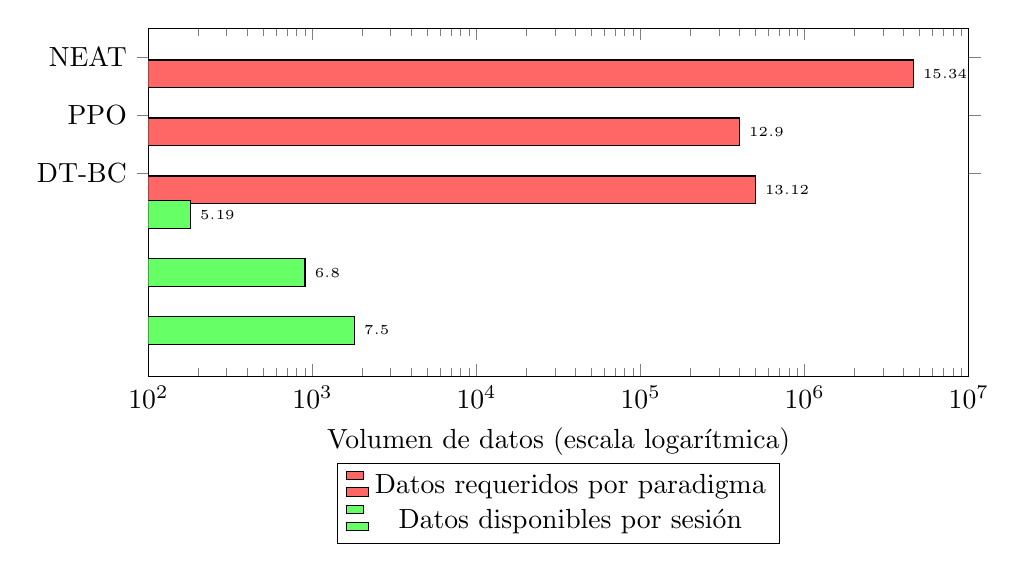
\begin{tikzpicture}
\begin{axis}[
    xbar,
    width=12cm, height=6cm,
    xlabel={Volumen de datos (escala logar\'{i}tmica)},
    symbolic y coords={{Sesi\'{o}n alta (100 part.)}, {Sesi\'{o}n media (50 part.)}, {Sesi\'{o}n baja (10 part.)}, DT-BC, PPO, NEAT},
    ytick=data,
    xmode=log,
    xmin=100, xmax=10000000,
    nodes near coords,
    nodes near coords align={horizontal},
    every node near coord/.append style={font=\tiny},
    bar width=10pt,
    legend style={at={(0.5,-0.25)}, anchor=north},
]
\addplot[fill=red!60] coordinates {(4590000,NEAT) (400000,PPO) (500000,DT-BC)};
\addplot[fill=green!60] coordinates {(1800,{Sesi\'{o}n alta (100 part.)}) (900,{Sesi\'{o}n media (50 part.)}) (180,{Sesi\'{o}n baja (10 part.)})};
\legend{Datos requeridos por paradigma, Datos disponibles por sesi\'{o}n}
\end{axis}
\end{tikzpicture}
\caption[Brecha de datos: entrenamiento vs.\ sesión real]{Brecha de datos entre los requerimientos de entrenamiento de cada paradigma y los datos disponibles en una sesi\'{o}n real contra un jugador humano (escala logar\'{i}tmica). Se observa una diferencia de 2 a 4 \'{o}rdenes de magnitud.}
\label{fig:brecha_datos}
\end{figure}

\subsection{Análisis de sensibilidad}

La estimación de 10--100 partidas por sesión debe interpretarse como un supuesto operativo conservador para el análisis de viabilidad, no como una medición formal de comportamiento de usuarios. Su función es establecer un orden de magnitud razonable para contrastar los requerimientos de entrenamiento. La Tabla~\ref{tab:sensibilidad} presenta tres escenarios que demuestran que la conclusión no cambia dentro de rangos razonables.

\begin{table}[H]
\centering
\caption{Análisis de sensibilidad: brecha de datos bajo tres escenarios de sesión humana}
\begin{tabular}{lccc}
\hline
\textbf{Escenario} & \textbf{Partidas} & \textbf{Muestras ($\sim$18 turnos)} & \textbf{Brecha vs PPO (400k)} \\
\hline
Bajo (pesimista)  & 10  & 180   & $\sim$2,222$\times$ \\
Medio             & 50  & 900   & $\sim$444$\times$ \\
Alto (optimista)  & 100 & 1,800 & $\sim$222$\times$ \\
\hline
\end{tabular}
\label{tab:sensibilidad}
\end{table}

Incluso en el escenario más optimista (100 partidas), la brecha es de más de dos órdenes de magnitud para PPO, el paradigma con menor requerimiento de datos entre los evaluados.

Adicionalmente, los experimentos con NEAT demostraron que el entrenamiento con datos insuficientes produce resultados aleatorios: con seed fija y 100 generaciones, NEAT no convergió (WR $\approx$ 0.50, equivalente a decisiones al azar). Solo cuando se garantizó diversidad y volumen suficiente de episodios (multi-seed real con 102 episodios por genoma) se alcanzó convergencia efectiva (WR = 0.626).

\subsection{Conclusión parcial}

El entrenamiento online continuo durante la partida, en hardware local, no es viable con los paradigmas evaluados debido a la escasez de datos, no solamente por restricciones de tiempo o recursos computacionales. Un jugador humano no genera suficientes muestras de interacción para que cualquiera de los tres enfoques converja a una política funcional.

\section{Calidad de Destilación PPO a DT}

La destilación por \textit{Behavior Cloning} \cite{hussein2017imitation} (aprendizaje supervisado imitando al PPO) produjo árboles de decisión con alta fidelidad al teacher, como se observa en la Tabla \ref{tab:distillation}:

\begin{table}[H]
\centering
\caption{Calidad de destilación: accuracy de los DT respecto al PPO teacher}
\begin{tabular}{lccc}
\hline
\textbf{DT destilado} & \textbf{Accuracy (\%)} & \textbf{Profundidad} & \textbf{Hojas} \\
\hline
dt\_ppo\_vs\_denial  & 93.79 & 10 & 773  \\
dt\_ppo\_vs\_spread  & 93.97 & 10 & 804  \\
dt\_ppo\_vs\_greedy  & 93.85 & 10 & 798  \\
\hline
\end{tabular}
\label{tab:distillation}
\end{table}

La destilación conserva $>$92\% de fidelidad al teacher PPO. Cada DT fue entrenado con $\sim$500,000 muestras generadas en 50,000 episodios de juego del PPO correspondiente.

\section{Perfilado KMeans}

El perfilador KMeans \cite{lloyd1982kmeans} se entrenó con datos de los 4 estilos heurísticos, usando una ventana temporal de 6 turnos. El perfil de cada oponente se representa mediante un vector de 10 dimensiones que captura patrones de decisión:

\begin{itemize}
    \item Histograma de columnas seleccionadas (3 dimensiones).
    \item Histograma de acciones legales disponibles (3 dimensiones).
    \item Proporción de selección de primera/última acción legal (2 dimensiones).
    \item Tasa de repetición de columna (1 dimensión).
    \item Entropía de la distribución de columnas (1 dimensión).
\end{itemize}

Este perfil de 10 dimensiones es independiente de las 21 features usadas por los agentes para seleccionar acciones; su propósito es caracterizar el \textit{estilo de juego} del oponente, no el estado del tablero.

El perfilador se configuró con los siguientes parámetros:

\begin{itemize}
    \item \textbf{k = 4} clusters (uno por cada estilo heurístico).
    \item \textbf{Silhouette score}: 0.232 (separación moderada, esperable dado que los estilos de juego comparten acciones en muchas situaciones).
    \item \textbf{Mapping cluster $\to$ estilo}: Cluster 0 $\to$ greedy, Cluster 1 $\to$ denial, Cluster 2 $\to$ denial, Cluster 3 $\to$ spread.
\end{itemize}

Se observa que 2 de 4 clusters fueron asignados al estilo \textit{denial}, lo que indica que el perfilador tiene dificultades para distinguir completamente entre todos los estilos. Esta limitación se analiza en detalle en la sección de Ablation Study.

\section{Evaluación de los Tres Sistemas Adaptativos}

Cada sistema adaptativo combina el perfilador KMeans compartido con una response table y tres especialistas de su paradigma. Se evaluaron los 3 sistemas contra los 3 oponentes heurísticos (5,000 partidas por matchup). Los resultados se presentan en la Tabla \ref{tab:systems_comparison}.

\begin{table}[H]
\centering
\caption{Winrate decidido de cada sistema vs cada oponente (5,000 partidas)}
\begin{tabular}{lcccc}
\hline
\textbf{Sistema} & \textbf{vs denial} & \textbf{vs spread} & \textbf{vs greedy} & \textbf{Promedio} \\
\hline
System NEAT & \textbf{0.635} & \textbf{0.697} & \textbf{0.626} & \textbf{0.653} \\
System DT   & 0.592          & 0.641          & 0.591          & 0.608 \\
System PPO  & 0.588          & 0.641          & 0.584          & 0.604 \\
\hline
\end{tabular}
\label{tab:systems_comparison}
\end{table}

El sistema NEAT alcanza un winrate promedio de 0.653 (IC 95\%: [0.645, 0.660]), significativamente superior a DT (0.608, IC: [0.600, 0.616]) y PPO (0.604, IC: [0.597, 0.612]). Este resultado se obtuvo tras implementar el entrenamiento multi-seed real, que mejoró la convergencia de NEAT.

\subsection{Resultados detallados por sistema}

A continuación se presentan los resultados desglosados de cada sistema adaptativo por oponente heurístico. Cada tabla muestra el número de partidas evaluadas, el winrate decidido (excluyendo empates), el intervalo de confianza al 95\%, el diferencial promedio de puntaje y el tiempo de ejecución.

\begin{table}[H]
\centering
\caption{System DT --- KMeans + Decision Trees destilados de PPO}
\begin{tabular}{lrccrc}
\hline
\textbf{Oponente} & \textbf{Games} & \textbf{WR decidido} & \textbf{IC 95\%} & \textbf{Avg diff} & \textbf{Wall (s)} \\
\hline
denial & 5,000 & 0.592 & [0.578, 0.606] & +4.80 & 30.4 \\
spread & 5,000 & 0.641 & [0.628, 0.654] & +8.06 & 40.0 \\
greedy & 5,000 & 0.591 & [0.577, 0.605] & +4.68 & 28.5 \\
\hline
\end{tabular}
\label{tab:system_dt}
\end{table}

\begin{table}[H]
\centering
\caption{System PPO --- KMeans + PPO especialistas directos}
\begin{tabular}{lrccrc}
\hline
\textbf{Oponente} & \textbf{Games} & \textbf{WR decidido} & \textbf{IC 95\%} & \textbf{Avg diff} & \textbf{Wall (s)} \\
\hline
denial & 5,000 & 0.588 & [0.574, 0.602] & +4.70 & 45.2 \\
spread & 5,000 & 0.641 & [0.628, 0.655] & +8.00 & 44.3 \\
greedy & 5,000 & 0.584 & [0.571, 0.598] & +4.50 & 43.1 \\
\hline
\end{tabular}
\label{tab:system_ppo}
\end{table}

\begin{table}[H]
\centering
\caption{System NEAT --- KMeans + NEAT especialistas directos (multi-seed)}
\begin{tabular}{lrccrc}
\hline
\textbf{Oponente} & \textbf{Games} & \textbf{WR decidido} & \textbf{IC 95\%} & \textbf{Avg diff} & \textbf{Wall (s)} \\
\hline
denial & 5,000 & 0.635 & [0.621, 0.648] & +6.40 & 28.8 \\
spread & 5,000 & 0.697 & [0.684, 0.710] & +11.0 & 27.4 \\
greedy & 5,000 & 0.626 & [0.613, 0.640] & +6.00 & 27.1 \\
\hline
\end{tabular}
\label{tab:system_neat}
\end{table}

\section{Análisis Estadístico entre Sistemas}

Se aplicó un \textbf{z-test de dos proporciones} (bilateral) a cada par de sistemas por oponente (9 comparaciones), con corrección de Bonferroni para comparaciones múltiples. Los valores $p$ se presentan en la Tabla \ref{tab:ztest}.

\begin{table}[H]
\centering
\caption{Valores p del z-test entre pares de sistemas (corregidos por Bonferroni)}
\begin{tabular}{lccc}
\hline
\textbf{Par comparado} & \textbf{vs denial ($p$)} & \textbf{vs spread ($p$)} & \textbf{vs greedy ($p$)} \\
\hline
DT vs PPO   & 1.000 & 1.000 & 1.000 \\
DT vs NEAT  & \textbf{0.0001} & \textbf{$<$0.0001} & \textbf{0.003} \\
PPO vs NEAT & \textbf{$<$0.0001} & \textbf{$<$0.0001} & \textbf{0.0002} \\
\hline
\end{tabular}
\label{tab:ztest}
\end{table}

\textbf{Resultado}: 6 de 9 comparaciones son estadísticamente significativas tras corrección de Bonferroni ($\alpha = 0.05$). El sistema NEAT es significativamente superior tanto a DT como a PPO en los tres oponentes evaluados. No se observa diferencia significativa entre DT y PPO. Las Figuras~\ref{fig:score_diff_dt}, \ref{fig:score_diff_ppo} y \ref{fig:score_diff_neat} muestran la distribución de los diferenciales de puntaje por paradigma, y la Figura~\ref{fig:score_diff_consolidated} presenta la comparativa consolidada de los sistemas adaptativos.

\begin{figure}[H]
\centering
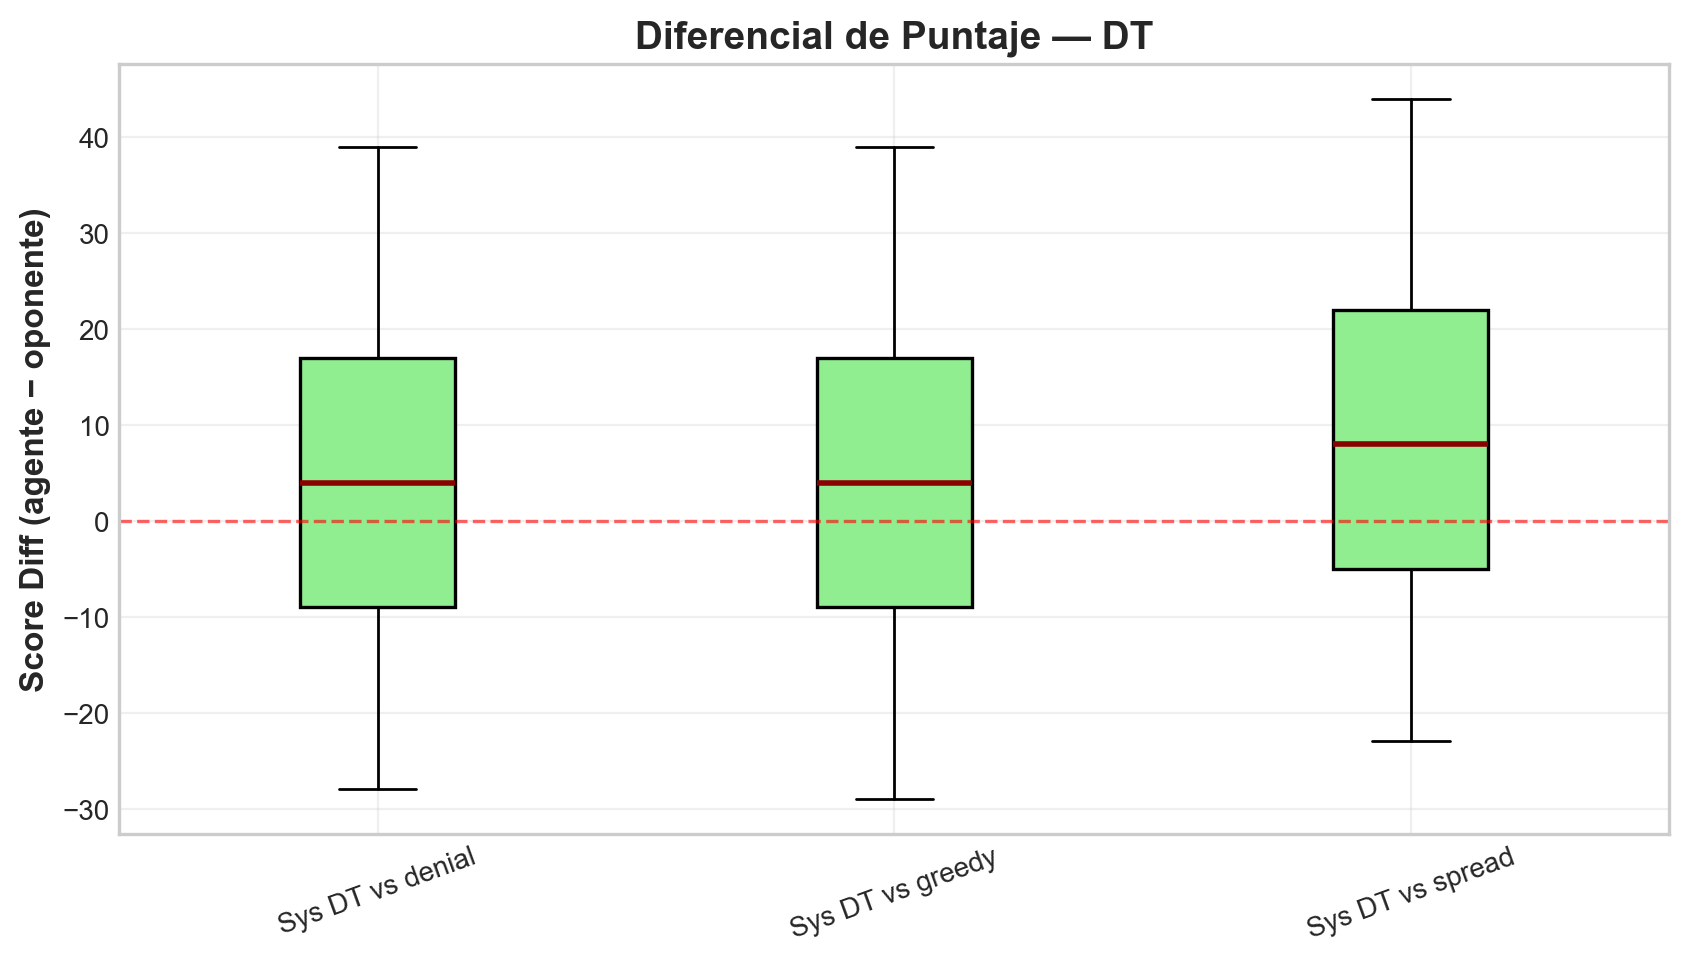
\includegraphics[width=0.85\textwidth]{figures/score_diff_dt.png}
\caption[Diferencial de puntaje --- DT]{Diferencial de puntaje para el paradigma DT (Decision Trees destilados). Las cajas representan percentiles p25--p75 y los bigotes p5--p95.}
\label{fig:score_diff_dt}
\end{figure}

\begin{figure}[H]
\centering
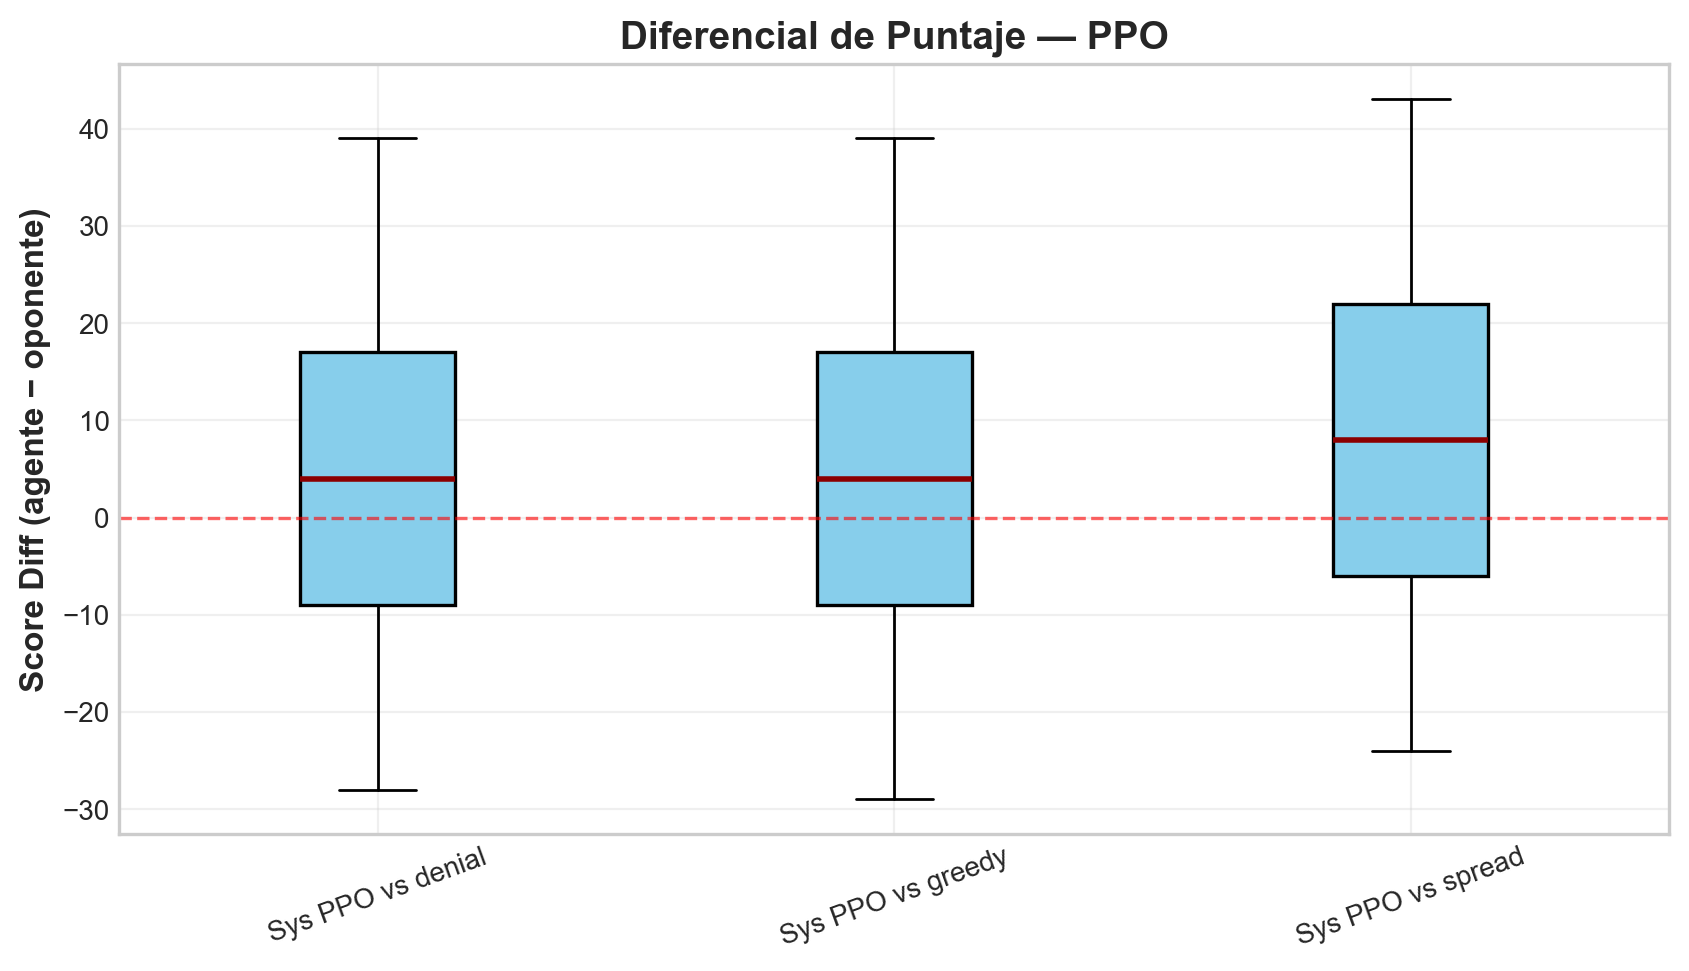
\includegraphics[width=0.85\textwidth]{figures/score_diff_ppo.png}
\caption[Diferencial de puntaje --- PPO]{Diferencial de puntaje para el paradigma PPO (Proximal Policy Optimization).}
\label{fig:score_diff_ppo}
\end{figure}

\begin{figure}[H]
\centering
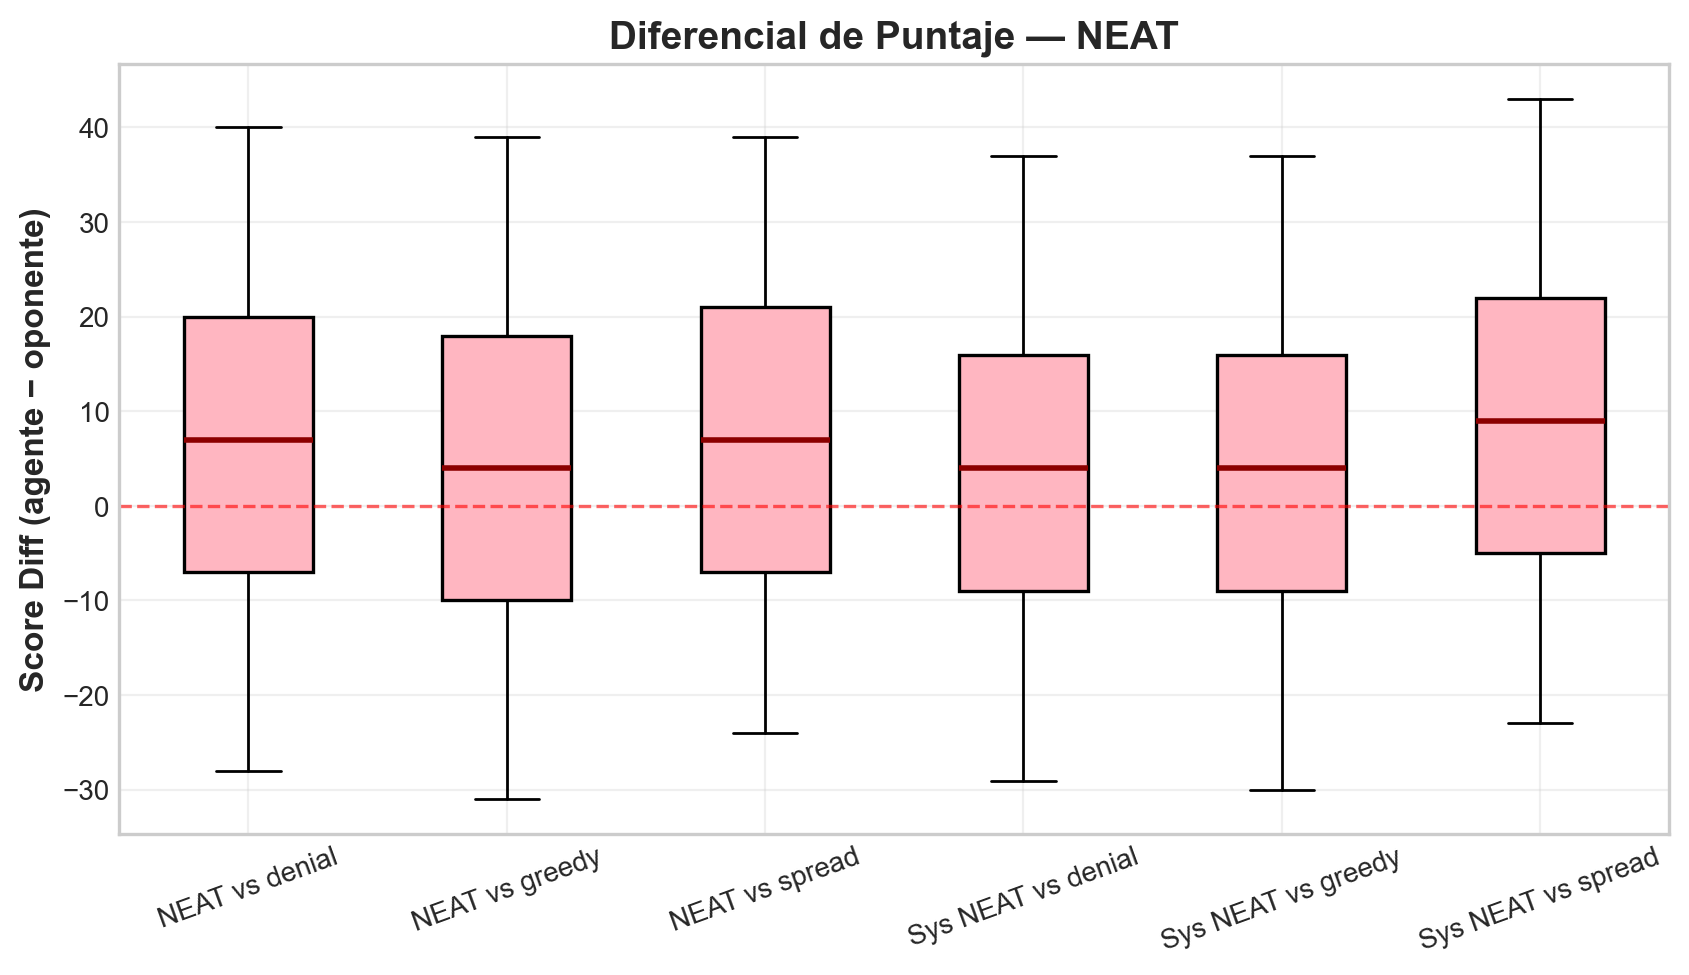
\includegraphics[width=0.85\textwidth]{figures/score_diff_neat.png}
\caption[Diferencial de puntaje --- NEAT]{Diferencial de puntaje para el paradigma NEAT (NeuroEvolution of Augmenting Topologies).}
\label{fig:score_diff_neat}
\end{figure}

\begin{figure}[H]
\centering
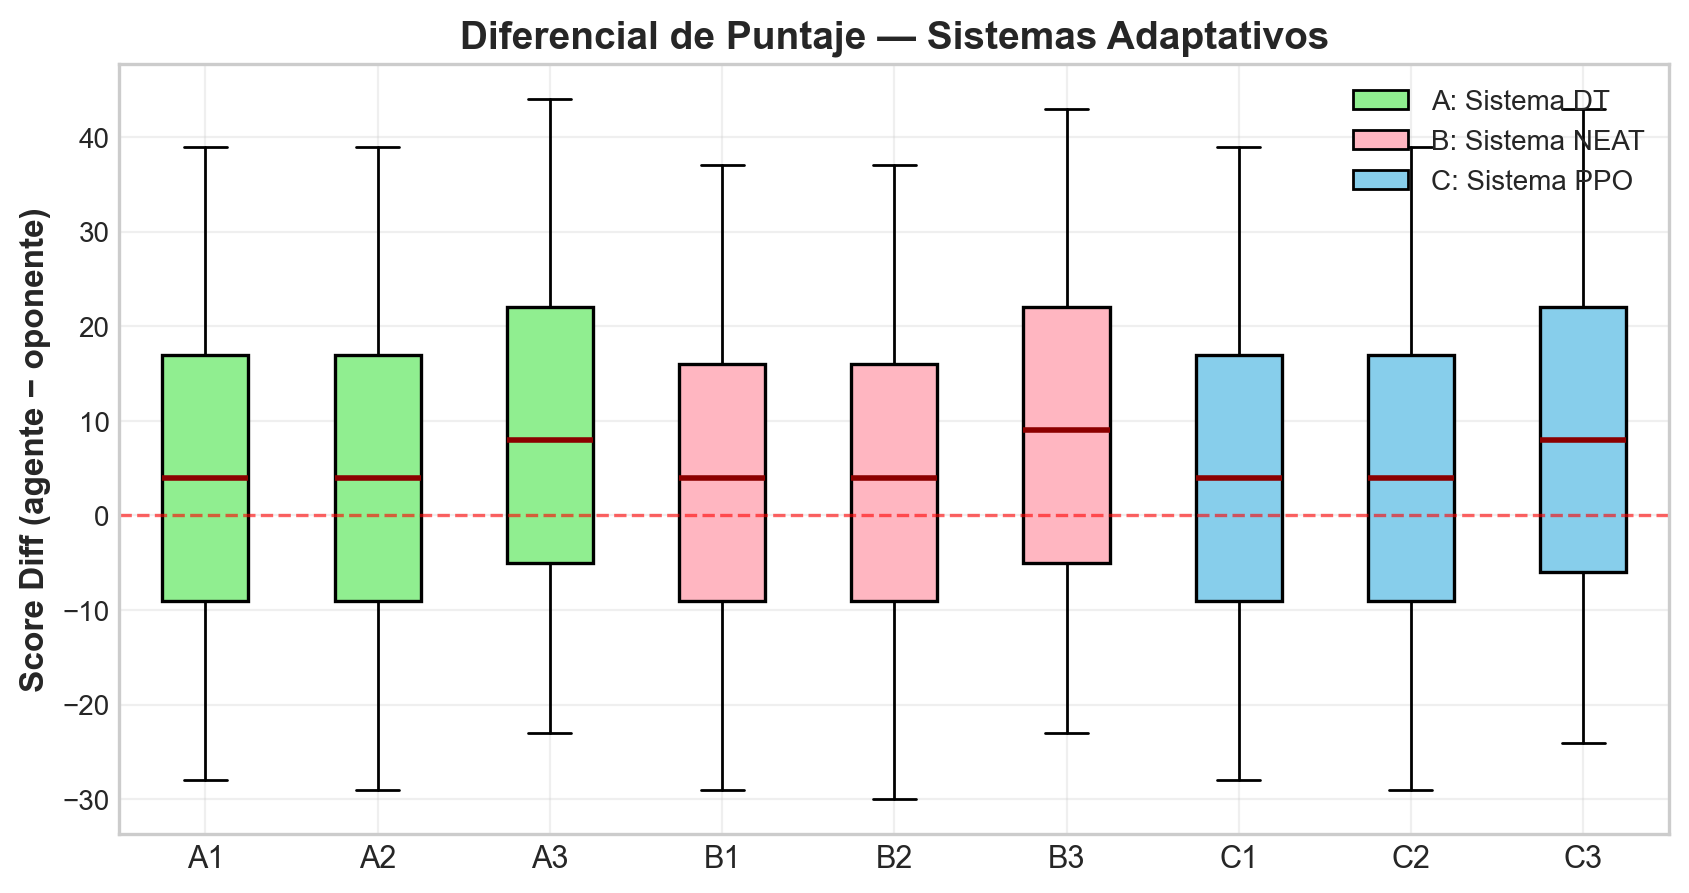
\includegraphics[width=0.9\textwidth]{figures/score_diff_boxplot.png}
\caption[Diferencial de puntaje --- Sistemas adaptativos]{Comparativa consolidada del diferencial de puntaje de los tres sistemas adaptativos. Variables: A = Sistema DT, B = Sistema NEAT, C = Sistema PPO. Subíndices: 1 = vs denial, 2 = vs greedy, 3 = vs spread. El sistema NEAT (rosa) muestra mayor ventaja promedio.}
\label{fig:score_diff_consolidated}
\end{figure}

\section{Ablation Study: ¿Aporta la Adaptación KMeans?}

Para cada familia se compararon cuatro condiciones, como se muestra en la Tabla \ref{tab:ablation}:

\begin{table}[H]
\centering
\caption{Ablation study: generalista vs adaptativo vs oráculo}
\begin{tabular}{lcccc}
\hline
\textbf{Familia} & \textbf{Peor gen.} & \textbf{Mejor gen.} & \textbf{Sistema adapt.} & \textbf{$\Delta$ Sist. vs Mejor} \\
\hline
DT   & 0.585 & 0.618 & 0.608 & $-$0.010 \\
PPO  & 0.572 & 0.610 & 0.604 & $-$0.005 \\
NEAT & 0.543 & \textbf{0.651} & \textbf{0.653} & +0.002  \\
\hline
\end{tabular}
\label{tab:ablation}
\end{table}

\textbf{Hallazgo clave}: el sistema adaptativo \textbf{no mejora} sobre el mejor generalista fijo en DT ($-$0.010 WR) y PPO ($-$0.005 WR). En NEAT muestra una mejora marginal (+0.002). Este resultado, lejos de invalidar el mecanismo de adaptación, lo posiciona como una alternativa operativamente viable: el mecanismo adaptativo es arquitectónicamente válido y mantiene rendimiento competitivo comparable al mejor generalista fijo, sin reentrenamiento en runtime y con costo computacional de inferencia despreciable (microsegundos). En Knucklebones, la baja diversidad estratégica del dominio limita el beneficio de la selección adaptativa; en juegos con mayor variedad de estilos de oponente se esperaría un beneficio más pronunciado.

La brecha de datos documentada en la sección anterior demuestra que el entrenamiento online no es una opción viable. La adaptación por selección cierra esta brecha al trasladar el costo del aprendizaje a la fase offline, manteniendo la capacidad de respuesta diferenciada en tiempo de ejecución.

\begin{enumerate}
    \item El KMeans asigna 2 de 4 clusters al estilo \textit{denial}, reduciendo su capacidad discriminante.
    \item Un solo especialista (entrenado vs greedy) resulta fuerte contra todos los oponentes.
    \item La response table ocasionalmente selecciona un especialista subóptimo para un cluster.
\end{enumerate}

\subsection{Dominancia en Response Tables}

La Tabla \ref{tab:dominance} muestra qué especialista fue seleccionado con mayor frecuencia por cada response table.

\begin{table}[H]
\centering
\caption{Dominancia de especialistas en las response tables}
\begin{tabular}{lcc}
\hline
\textbf{Sistema} & \textbf{Especialista dominante} & \textbf{Cobertura} \\
\hline
System DT   & dt\_vs\_denial    & 2/4 (50\%)  \\
System PPO  & PPO\_vs\_denial        & 2/4 (50\%)  \\
System NEAT & neat\_vs\_denial       & 4/4 (100\%) \\
\hline
\end{tabular}
\label{tab:dominance}
\end{table}

\textbf{Interpretación}: el mecanismo adaptativo es arquitectónicamente válido, pero en Knucklebones los estilos no son suficientemente distintos para que la selección diferenciada aporte mejora competitiva significativa. En DT y PPO se utilizan 3 especialistas distintos (uno por estilo dominante en cada cluster), mientras que en NEAT un solo especialista (denial) domina todos los clusters, indicando que aprendió una política generalista fuerte. En juegos con mayor diversidad estratégica se esperaría una distribución más equilibrada entre especialistas.

\textit{Nota}: los datos de esta tabla fueron extraídos directamente de los archivos de response table generados por \texttt{build\_response\_table.py}, los cuales registran la selección óptima de especialista por cluster según winrate decidido.

\section{Evaluación Cruzada: Generalización vs Sobreajuste}

Cada especialista se evaluó contra \textbf{todos} los oponentes (2,000 partidas por matchup) para detectar sobreajuste. El símbolo $\star$ indica el oponente contra el que fue entrenado. Los resultados por familia se presentan en las Tablas \ref{tab:cross_neat}, \ref{tab:cross_ppo} y \ref{tab:cross_dt}, con un resumen de generalización en la Tabla \ref{tab:generalization}.

\begin{table}[H]
\centering
\caption{Evaluación cruzada de NEAT especialistas (winrate decidido)}
\begin{tabular}{lccc}
\hline
\textbf{Especialista} & \textbf{vs denial} & \textbf{vs spread} & \textbf{vs greedy} \\
\hline
NEAT $\to$ denial & 0.635$\star$ & 0.692 & 0.627 \\
NEAT $\to$ spread & 0.496 & 0.634$\star$ & 0.499 \\
NEAT $\to$ greedy & 0.635 & 0.692 & 0.627$\star$ \\
\hline
\end{tabular}
\label{tab:cross_neat}
\end{table}

Se observa que los especialistas NEAT entrenados contra denial y greedy convergen a políticas similares, ambas generalistas fuertes (WR $>$ 0.62 contra todos los oponentes). En contraste, el especialista entrenado contra spread presenta bajo rendimiento generalista.

\begin{table}[H]
\centering
\caption{Evaluación cruzada de PPO especialistas (winrate decidido)}
\begin{tabular}{lccc}
\hline
\textbf{Especialista} & \textbf{vs denial} & \textbf{vs spread} & \textbf{vs greedy} \\
\hline
PPO $\to$ denial & 0.598$\star$ & 0.625 & 0.589 \\
PPO $\to$ spread & 0.531 & 0.650$\star$ & 0.535 \\
PPO $\to$ greedy & 0.600 & 0.626 & 0.602$\star$ \\
\hline
\end{tabular}
\label{tab:cross_ppo}
\end{table}

Los especialistas PPO muestran un patrón similar: el entrenado contra greedy es el mejor generalista, mientras que el de spread es el más especializado.

\begin{table}[H]
\centering
\caption{Evaluación cruzada de DT especialistas (winrate decidido)}
\begin{tabular}{lccc}
\hline
\textbf{Especialista} & \textbf{vs denial} & \textbf{vs spread} & \textbf{vs greedy} \\
\hline
DT $\to$ denial & 0.589$\star$ & 0.633 & 0.589 \\
DT $\to$ spread & 0.549 & 0.656$\star$ & 0.548 \\
DT $\to$ greedy & 0.601 & 0.651 & 0.601$\star$ \\
\hline
\end{tabular}
\label{tab:cross_dt}
\end{table}

Los DT destilados heredan el comportamiento de sus teachers PPO, mostrando patrones de generalización similares. La Tabla~\ref{tab:generalization} resume los resultados de generalización de las tres familias.

\begin{table}[H]
\centering
\caption{Resumen de generalización por familia}
\begin{tabular}{lcc}
\hline
\textbf{Familia} & \textbf{$\Delta$ promedio} & \textbf{Veredicto} \\
\hline
NEAT & +0.007 & Sin sobreajuste \\
PPO  & +0.018 & Sin sobreajuste \\
DT   & +0.010 & Sin sobreajuste \\
\hline
\end{tabular}
\label{tab:generalization}
\end{table}

\textbf{Hallazgos}:

\begin{enumerate}
    \item No se detecta sobreajuste ($\Delta < 3\%$ en todas las familias).
    \item Spread es el oponente más ``fácil'' ($\sim$0.63--0.69 independientemente del entrenamiento).
    \item NEAT\_vs\_denial y NEAT\_vs\_greedy convergen a políticas generalistas fuertes con multi-seed (WR $>$ 0.62 contra todo).
    \item NEAT\_vs\_spread sigue siendo el más débil, mostrando que el estilo de entrenamiento importa.
    \item Los especialistas entrenados contra greedy son los mejores generalistas en PPO y DT.
\end{enumerate}

La Figura~\ref{fig:cross_eval_heatmap} presenta visualmente los resultados de la evaluación cruzada mediante un mapa de calor, donde se observa claramente que los especialistas entrenados contra spread tienen menor capacidad de generalización.

\begin{figure}[H]
\centering
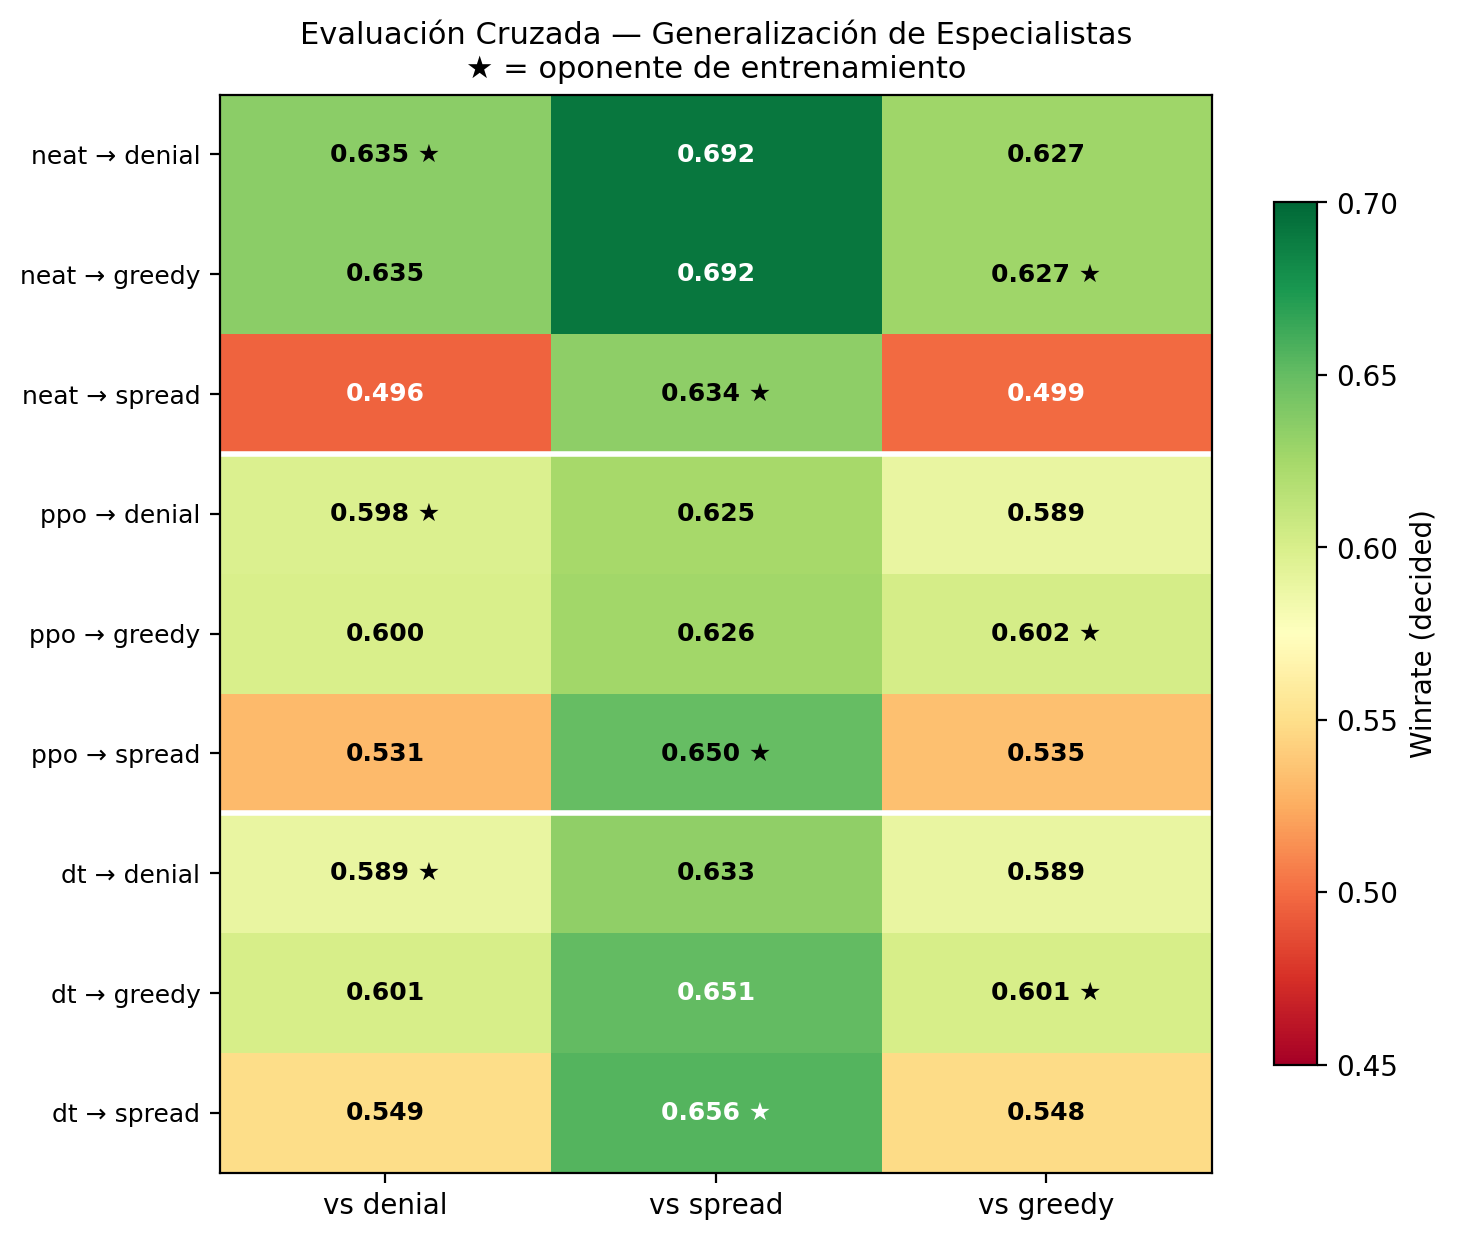
\includegraphics[width=0.85\textwidth]{figures/cross_eval_heatmap.png}
\caption[Mapa de calor de evaluación cruzada]{Mapa de calor de la evaluación cruzada: cada especialista (fila) evaluado contra todos los oponentes (columna). Colores más cálidos indican mayor winrate. Se observa que los especialistas entrenados contra greedy y denial generalizan mejor que los entrenados contra spread.}
\label{fig:cross_eval_heatmap}
\end{figure}

\section{NEAT: Convergencia, Entrenamiento Extendido y Multi-seed}

Se investigó la sensibilidad de NEAT a la convergencia y la prevención de sobreajuste a secuencias deterministas. Se compararon tres enfoques, cuyos resultados se presentan en la Tabla \ref{tab:neat_extended}:

\begin{table}[H]
\centering
\caption{Efecto de la estrategia de entrenamiento en NEAT vs greedy}
\begin{tabular}{lccc}
\hline
\textbf{Variante} & \textbf{WR decidido} & \textbf{Generaciones} & \textbf{Tiempo (min)} \\
\hline
Original (seed fija)           & 0.499 & 100        & $\sim$12  \\
Extended (seed rotation)       & 0.582 & 1,000      & $\sim$100 \\
Multi-seed real (3 seeds)      & \textbf{0.626} & 300 & $\sim$30  \\
\hline
\end{tabular}
\label{tab:neat_extended}
\end{table}

El enfoque multi-seed real evalúa cada genoma contra 3 seeds simultáneamente en cada generación, promediando el fitness. Este método alcanzó el mejor rendimiento (WR = 0.626) en el menor tiempo ($\sim$30 minutos), superando tanto al entrenamiento original que no convergió (WR $\approx$ 0.50) como al extended con seed rotation (WR = 0.582, 100 minutos).

Test z (multi-seed vs original): $z = 8.97$, $p < 0.0001$ $\to$ \textbf{diferencia estadísticamente significativa}.

La Figura~\ref{fig:neat_evolution} muestra la evolución del fitness durante el entrenamiento de NEAT multi-seed real, evidenciando la convergencia progresiva del algoritmo.

\begin{figure}[H]
\centering
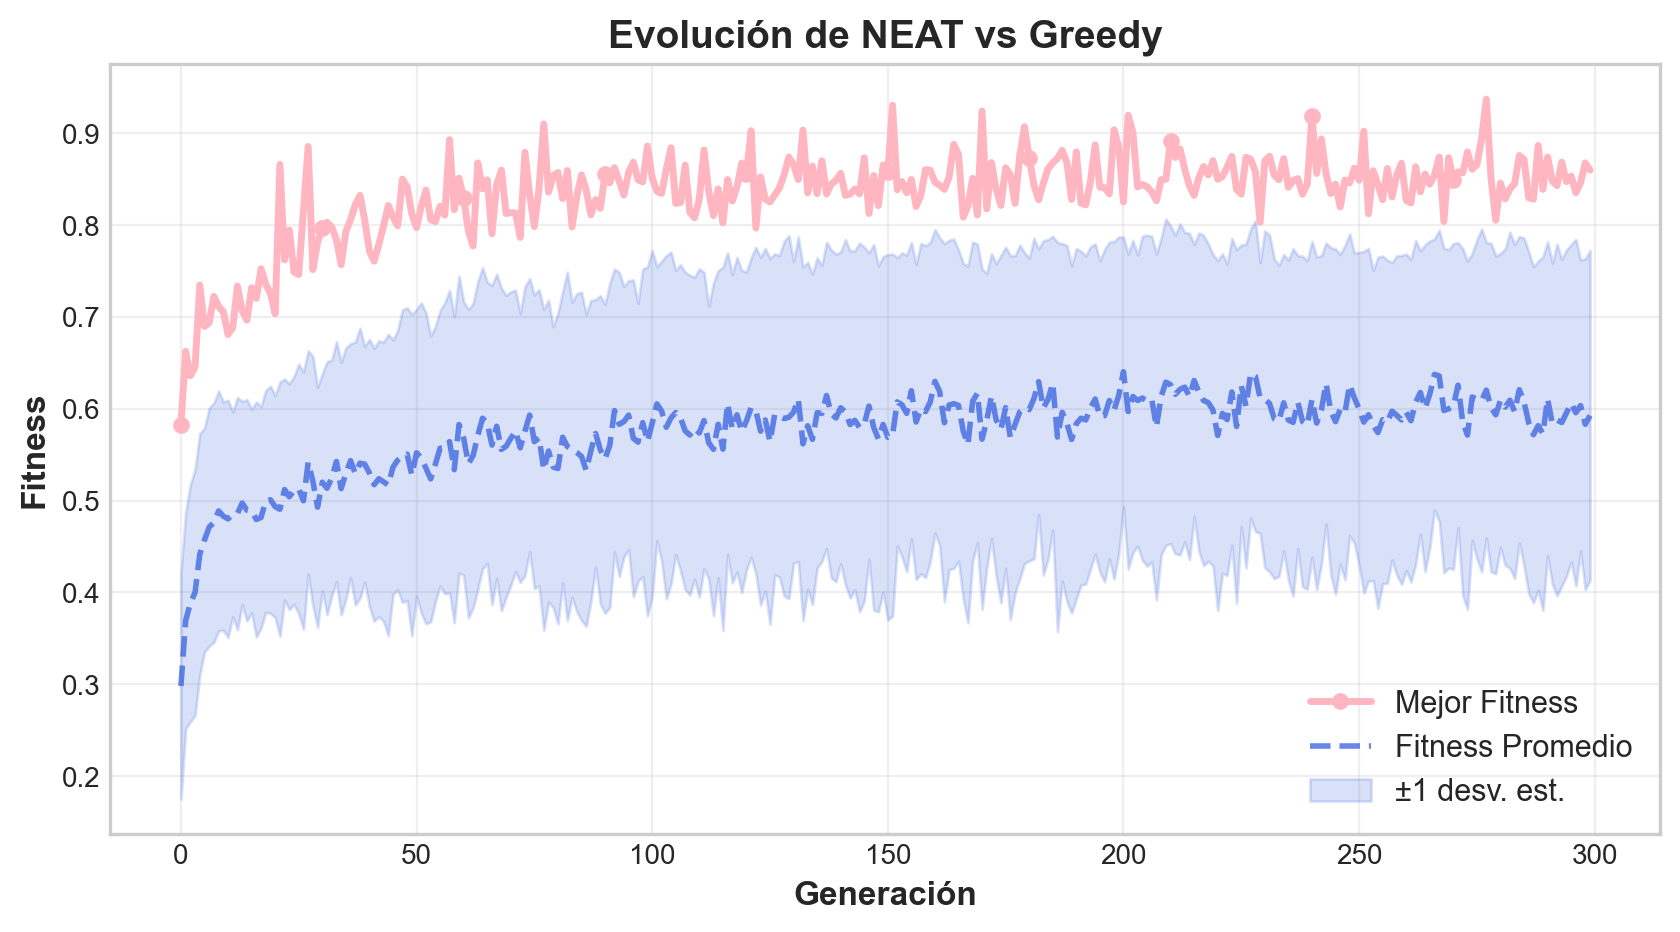
\includegraphics[width=0.75\textwidth]{figures/neat_evolution_heuristic_greedy.png}
\caption[Evolución de fitness NEAT multi-seed]{Evolución del fitness de NEAT multi-seed real vs greedy durante 300 generaciones. Se observa convergencia progresiva sin sobreajuste.}
\label{fig:neat_evolution}
\end{figure}

La mejora se extiende a todos los oponentes: contra denial pasó de WR = 0.565 a 0.635 (+7\%), y contra spread se mantuvo estable en 0.634. Este hallazgo demuestra que la técnica de entrenamiento (multi-seed real) tiene mayor impacto que la cantidad de generaciones.

\section{Discusión}

\subsection{Comparativa consolidada de paradigmas}

La Tabla \ref{tab:paradigm_comparison} presenta una comparativa consolidada de los tres paradigmas evaluados, considerando rendimiento competitivo, costo computacional y características cualitativas.

\begin{table}[H]
\centering
\caption{Comparativa de paradigmas: rendimiento vs costo}
\begin{tabular}{lcccccc}
\hline
\textbf{Criterio} & \textbf{PPO} & \textbf{NEAT} & \textbf{DT (destilado)} \\
\hline
Winrate promedio & 0.604 & \textbf{0.653} & 0.608 \\
Inferencia (5k juegos) & 44s & 28s & \textbf{33s} \\
Tamaño modelo & 161 KB & \textbf{3.4 KB} & 145 KB \\
Entrenamiento & $\sim$10 min & $\sim$30 min & $<$3s (+PPO) \\
¿Requiere tuning? & No & Sí & No \\
¿Interpretable? & No & No & \textbf{Sí} \\
GPU necesaria & No & No & No \\
\hline
\end{tabular}
\label{tab:paradigm_comparison}
\end{table}

La Figura~\ref{fig:comparativa_paradigmas} presenta de forma visual la comparativa de winrate promedio de cada paradigma, y la Figura~\ref{fig:system_winrates} muestra los winrates agrupados por sistema y oponente.

\begin{figure}[H]
\centering
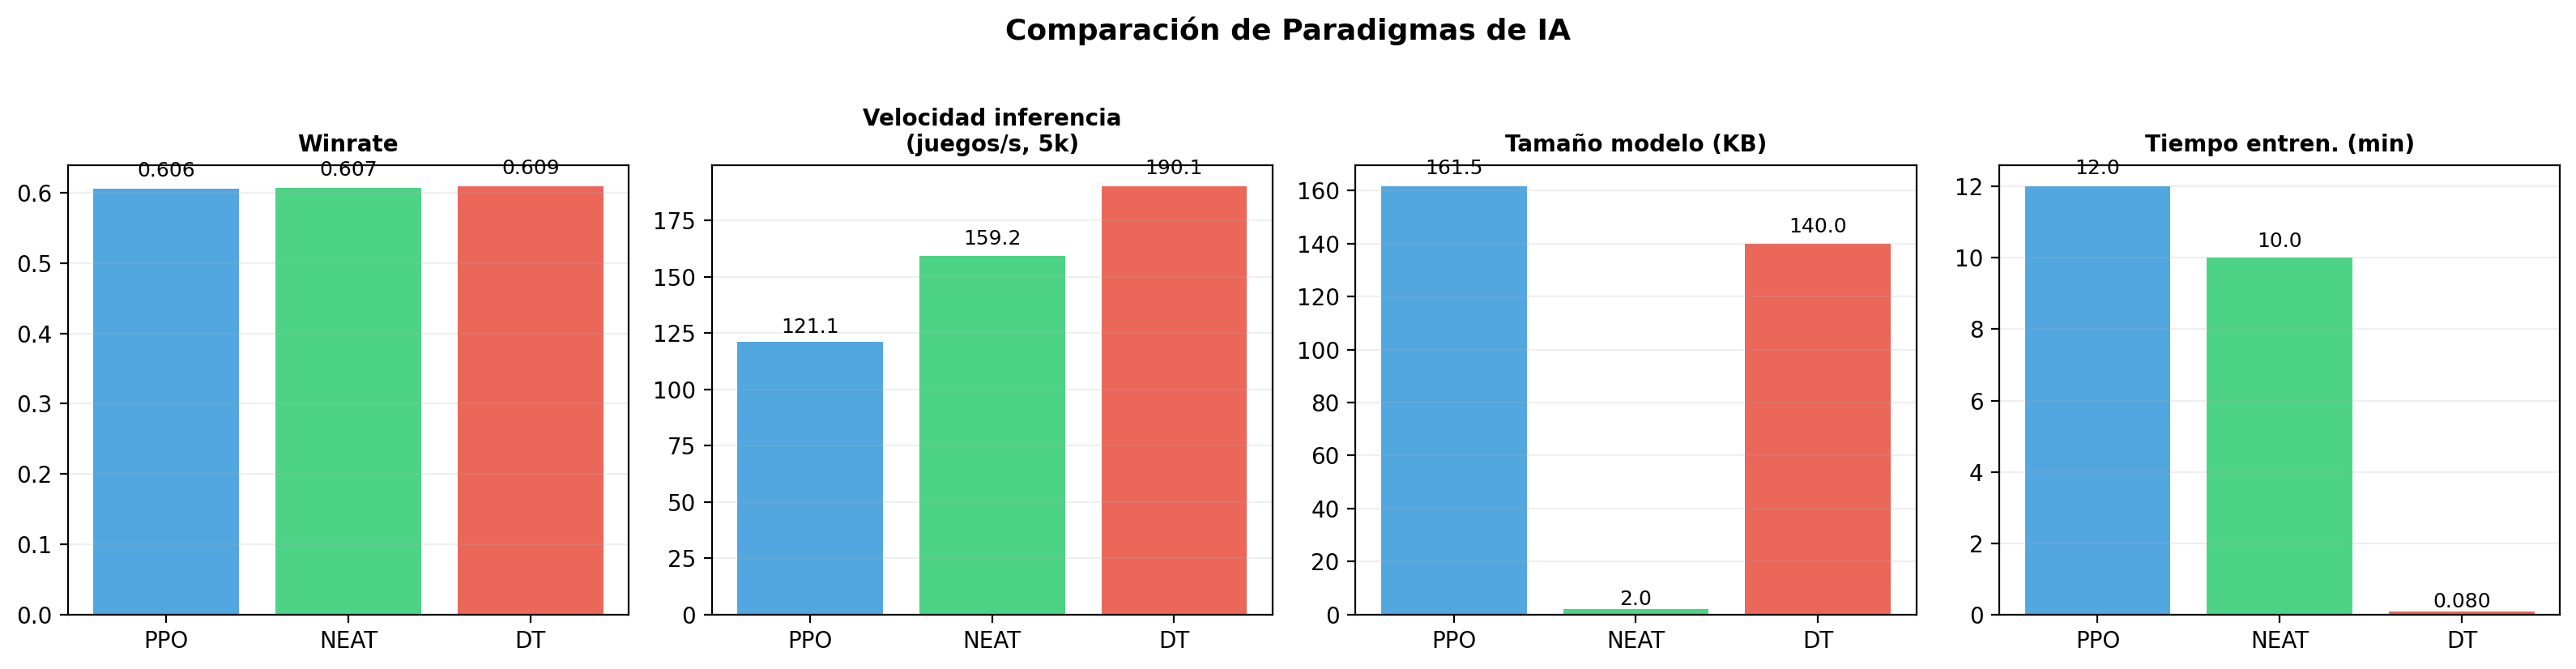
\includegraphics[width=0.8\textwidth]{figures/paradigm_comparison.png}
\caption[Comparativa consolidada de paradigmas]{Comparativa consolidada de paradigmas: winrate promedio, tiempo de entrenamiento y tamaño de modelo.}
\label{fig:comparativa_paradigmas}
\end{figure}

\begin{figure}[H]
\centering
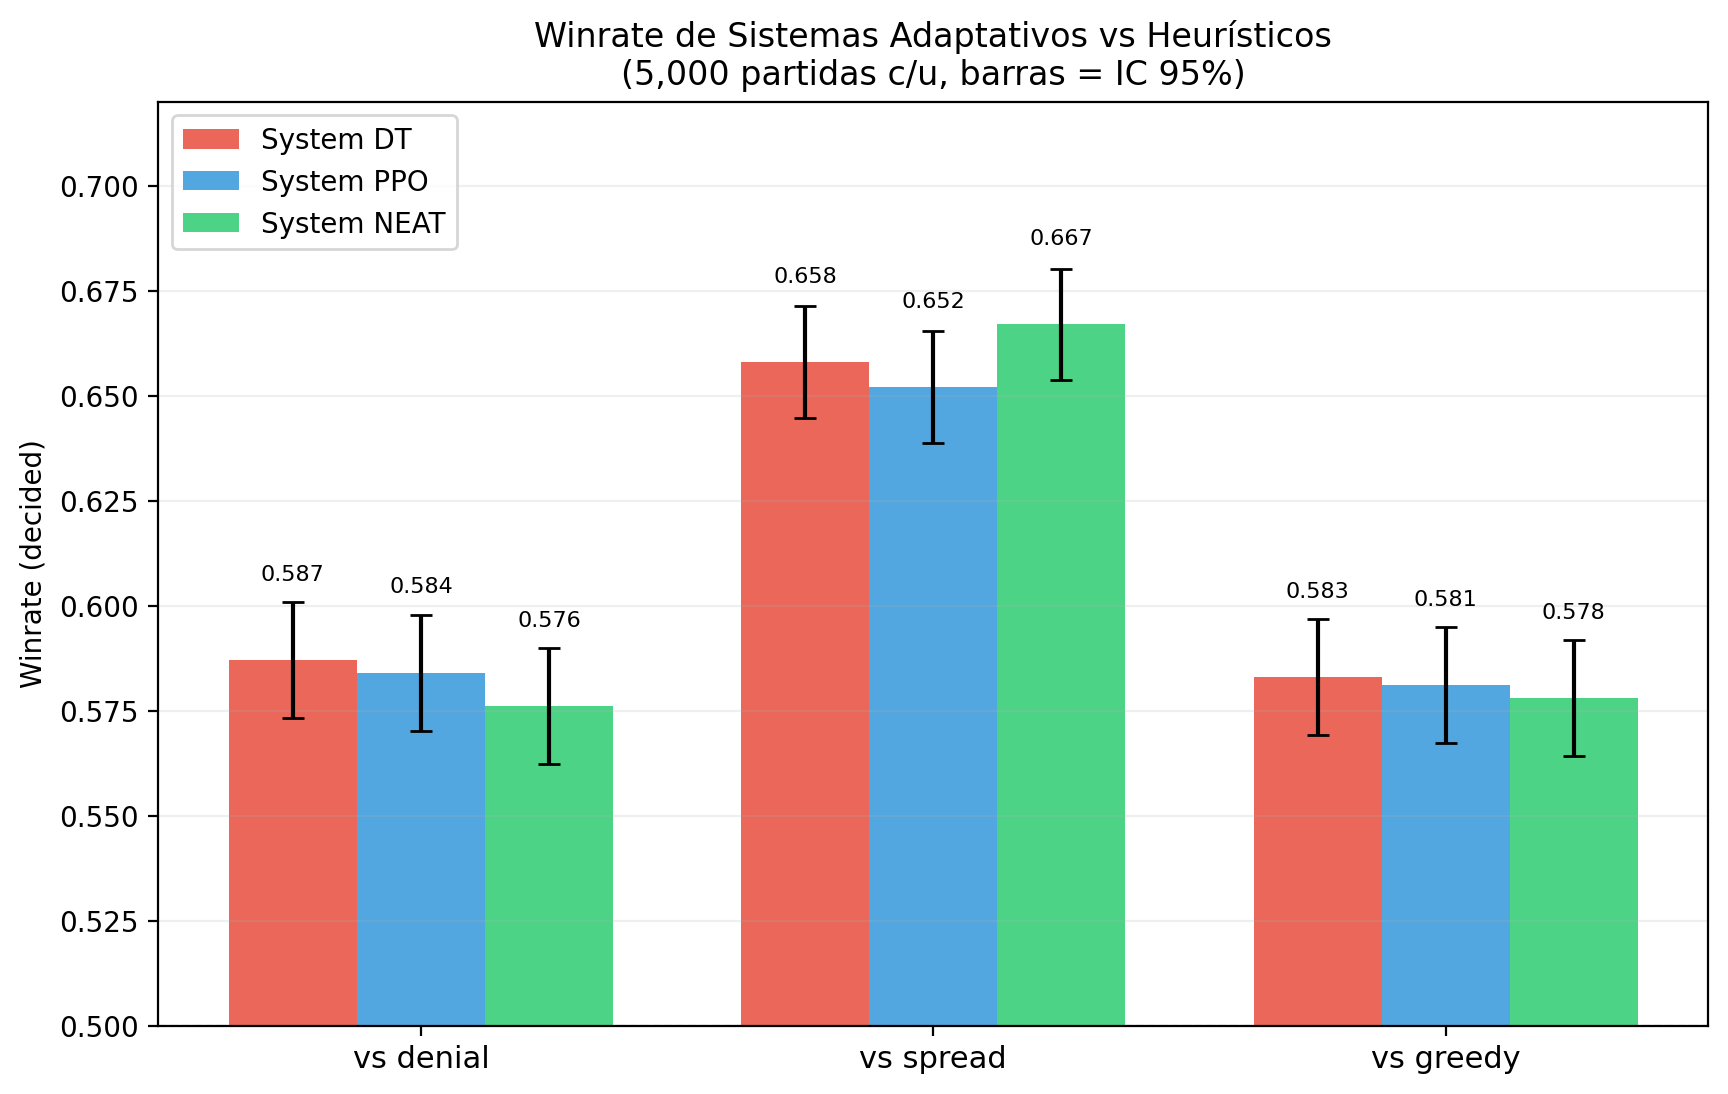
\includegraphics[width=0.8\textwidth]{figures/system_winrates_grouped.png}
\caption[Winrate por sistema y oponente]{Winrate de cada sistema adaptativo por oponente heurístico (5,000 partidas por matchup).}
\label{fig:system_winrates}
\end{figure}

\subsection{Hallazgos principales}

\begin{enumerate}
    \item \textbf{El entrenamiento en tiempo real no es viable por escasez de datos}: los tres paradigmas requieren entre 2 y 4 órdenes de magnitud más datos de los que un jugador humano genera en una sesión real (180--1,800 muestras vs. 400,000--4,590,000 requeridas). Esta brecha no se resuelve con mayor velocidad de cómputo.

    \item \textbf{El entrenamiento offline en hardware local sí es viable}: todos los modelos se entrenaron en $<$33 minutos por especialista, sin GPU, en hardware doméstico. El pipeline completo (entrenamiento + evaluación) se ejecuta en menos de 3 horas. Esto demuestra que el aprendizaje es factible cuando se dispone de un entorno de simulación acelerada.

    \item \textbf{La adaptación por selección es operativamente viable}: el mecanismo de KMeans + response table + especialistas pre-entrenados mantiene rendimiento competitivo comparable al mejor generalista fijo, con latencia de inferencia del agente inferior a 0.1 ms por turno y sin reentrenamiento en runtime. Su beneficio competitivo es limitado en Knucklebones debido a la baja diversidad estratégica del dominio.

    \item \textbf{NEAT con multi-seed alcanza el mejor rendimiento}: con WR = 0.653 (IC 95\%: [0.645, 0.660]), el sistema NEAT supera significativamente a PPO (0.604) y DT (0.608), con $p < 0.003$ en 6 de 9 comparaciones tras corrección de Bonferroni. La técnica de entrenamiento multi-seed real fue determinante para la convergencia.

    \item \textbf{La destilación preserva el rendimiento en un modelo ligero}: PPO y DT destilado son estadísticamente equivalentes ($p > 0.5$), demostrando que \textit{Behavior Cloning} preserva $>$93\% de fidelidad con un modelo interpretable, inferencia más rápida y entrenamiento instantáneo ($<$3 segundos). Esto evidencia una ruta viable para comprimir modelos entrenados offline.

    \item \textbf{Ausencia de sobreajuste}: $\Delta < 2\%$ en evaluación cruzada para todas las familias. Los agentes generalizan contra oponentes no vistos durante el entrenamiento.
\end{enumerate}

\subsection{Implicaciones}

\textbf{Sobre el aprendizaje en tiempo real}: los resultados demuestran que el entrenamiento online continuo durante la partida no es viable en hardware local con los paradigmas evaluados (PPO, NEAT, DT). La limitación principal no es la capacidad de cómputo, sino la escasez fundamental de datos: un jugador humano genera órdenes de magnitud menos muestras de las necesarias para que cualquiera de estos enfoques converja.

\textbf{Sobre la adaptación por selección}: el mecanismo de perfilado (KMeans) combinado con selección de especialistas pre-entrenados constituye una alternativa práctica demostrada. No requiere reentrenamiento en runtime, opera con latencia despreciable ($<$0.1 ms) y alcanza un rendimiento competitivo equivalente al mejor generalista fijo. En dominios con mayor diversidad estratégica (RTS, MOBA), donde un solo agente generalista no puede cubrir todos los perfiles de oponente, se esperaría un beneficio más pronunciado de este mecanismo.

\textbf{Sobre la elección de paradigma}: cuando el entrenamiento offline es la vía elegida, NEAT con multi-seed real ofrece el mejor rendimiento competitivo (WR = 0.653) con modelos ultraligeros (3.4 KB). Si se prioriza interpretabilidad o velocidad de iteración, DT destilado por \textit{Behavior Cloning} ofrece rendimiento equivalente a PPO con entrenamiento casi instantáneo.

\subsection{Limitaciones observadas}

\begin{itemize}
    \item \textbf{Dominio experimental limitado}: Knucklebones es un juego de reglas simples con espacio de acciones reducido (3 columnas). La brecha de datos podría variar en juegos con mayor complejidad, aunque probablemente se ampliaría dado que dominios más complejos requieren más datos de entrenamiento.
    \item \textbf{Oponentes heurísticos}: los oponentes de entrenamiento y evaluación son heurísticos diseñados, no jugadores humanos reales. Un estudio con jugadores humanos aportaría validez externa adicional.
    \item \textbf{Paradigmas evaluados}: se evaluaron tres paradigmas representativos (RL, neuroevolución, aprendizaje supervisado). Existen enfoques no evaluados ---como \textit{meta-learning}, \textit{few-shot learning} o aprendizaje incremental--- que podrían reducir la brecha de datos, aunque su aplicabilidad en videojuegos en hardware local permanece como pregunta abierta.
    \item \textbf{Sesión humana estimada}: la estimación de 10--100 partidas como límite de una sesión humana se basa en observación práctica y no en un estudio formal de comportamiento de usuario.
    \item \textbf{KMeans con k fijo}: no se exploró exhaustivamente el espacio de hiperparámetros del perfilador. Un clustering más fino podría mejorar la selección de especialistas.
\end{itemize}

